%Beamer class
\documentclass{beamer}

\usepackage[czech]{babel}
\usepackage[utf8]{inputenc}
\usepackage{fontenc}
\usepackage{tgheros}
\usepackage{array}
\usepackage{color}
\usepackage{hyperref}

\usetheme{AnnArbor}
\usecolortheme{crane}


\title[Realizace prototypu]{Realizace prototypu}
\subtitle[KEO] {Konstrukce a realizace elektronických obvodů}
\author[Brejcha]{\texorpdfstring{Michal Brejcha\newline\url{brejcmic@fel.cvut.cz}}{Michal Brejcha}}
\institute[ČVUT]{ČVUT v Praze, FEL}
\date[Praha, 2023]{Praha, 2023}

%------------------------------------------------------------------------------
%Konstanty a definice
%------------------------------------------------------------------------------
\newtheorem{myDef}{}

\begin{document}
%------------------------------------------------------------------------------
%Uvodni slajd
%------------------------------------------------------------------------------
\frame{\titlepage}

\begin{frame}
\frametitle{Obsah} 
\tableofcontents
\end{frame}

\AtBeginSection[]
{
  \begin{frame}
    \frametitle{Téma}
    \tableofcontents[currentsection]
  \end{frame}
}

%------------------------------------------------------------------------------
%Návrh
%------------------------------------------------------------------------------
\section{\texorpdfstring{Základní materiály DPS}{Základní materiály DPS}}
%------------------------------------------------------------------------------
\begin{frame}
	\frametitle{Deska plošného spoje}
	
	Propojovací cesty jsou vytvářeny pomocí napařené měděné folie na dielektrickém substrátu. 

	\begin{center}
		\begin{tabular}{p{0.2\linewidth} p{0.7\linewidth}}
		Vodič: & Cu Folie. Tloušťka je značena v oz (unce - hmotnostní jednotka). 1~oz$\approx$35~$\mu$m, nejběžnější tloušťky jsou 0.5~oz, 1~oz a 2~oz.\\ \\
		Izolant: & skelná tkanina $+$ epoxydová pryskyřice. Existují v zásadě různé materiály lišící se poměrem objemu tkaniny ku pryskyřici čímž lze měnit dielektrické i mechanické vlastnosti.
		
		Základní vlastnosti:
		
		\begin{itemize}
			\item $\epsilon_r\approx 3.8 - 5$,
			\item $E_{max}\approx 15$~kV/mm,
		\end{itemize}
		\end{tabular}
	\end{center}
\end{frame}
%------------------------------------------------------------------------------
\begin{frame}
	\frametitle{Měděná folie}
	
	
	\begin{center}
		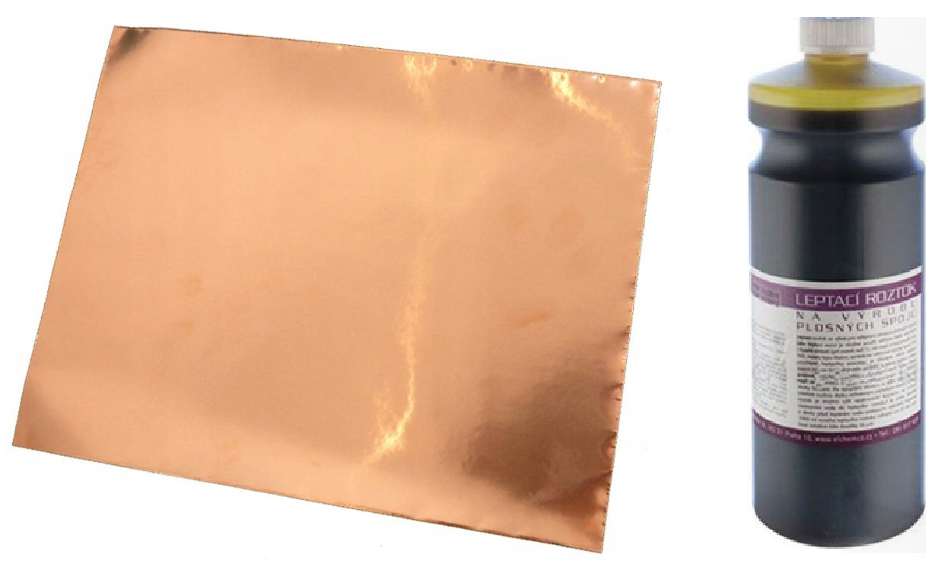
\includegraphics[width=0.38\textwidth]{CU.png}
	\end{center}
	
	\begin{itemize}
		\item malý odpor, pro 1 oz je zhruba $R_{sq}= 1$ m$\Omega$/ čtverec,
		\item ušlechtilý kov,
		\item rozpouští se v roztoku chloridu železitého ($FeCl_3$)
	\end{itemize}
	\textbf{Výpočet odporu vodivé cesty:}
	
		\[
		R= n \cdot R_{sq} = \frac{l}{w} \cdot R_{sq}
	\]
	\small
	$n$... počet čtverců, $l$... délka cesty, $w$... šířka cesty
	
\end{frame}
%------------------------------------------------------------------------------
\begin{frame}
	\frametitle{Sklolaminátová deska FR4}
	
	
	\begin{center}
		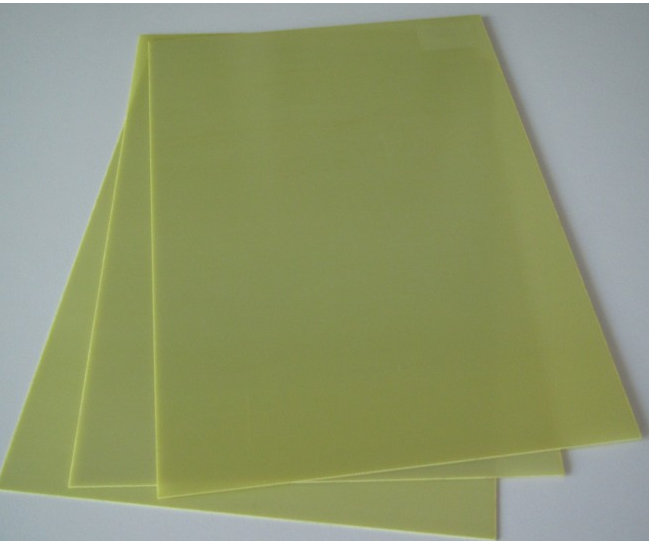
\includegraphics[width=0.30\textwidth]{FR4.png}
	\end{center}
	
	\begin{itemize}
		\item stabilní elektrické izolační vlastnosti $E_{max}> 15$~kV/mm,
		\item hladký povrch,
		\item vysoká pevnost v tlaku, ohybu: obvykle $>500$~MPa (PTFE $\approx 14$~MPa),
		\item vysoká pevnost v tahu: obvykle $>250$~MPa (PTFE $\approx 12$~MPa),
		\item srovnatelná hustota s plasty: $\approx 2000$~kg/m$^3$ (PTFE $\approx 2200$~kg/m$^3$, PVC $\approx 1400$~kg/m$^3$),
		\item nízká navlhavost, nehořlavost a dobrá chemická odolnost,
		\item teplotní odolnost do cca $140^\circ$C
		
	\end{itemize}
	
\end{frame}

%------------------------------------------------------------------------------
\section{\texorpdfstring{Výroba DPS}{Výroba DPS}}
%------------------------------------------------------------------------------
\begin{frame}
	\frametitle{Jádro PCB}
	
	\begin{center}
			\begin{tabular}{m{0.4\linewidth} m{0.5\linewidth}}
			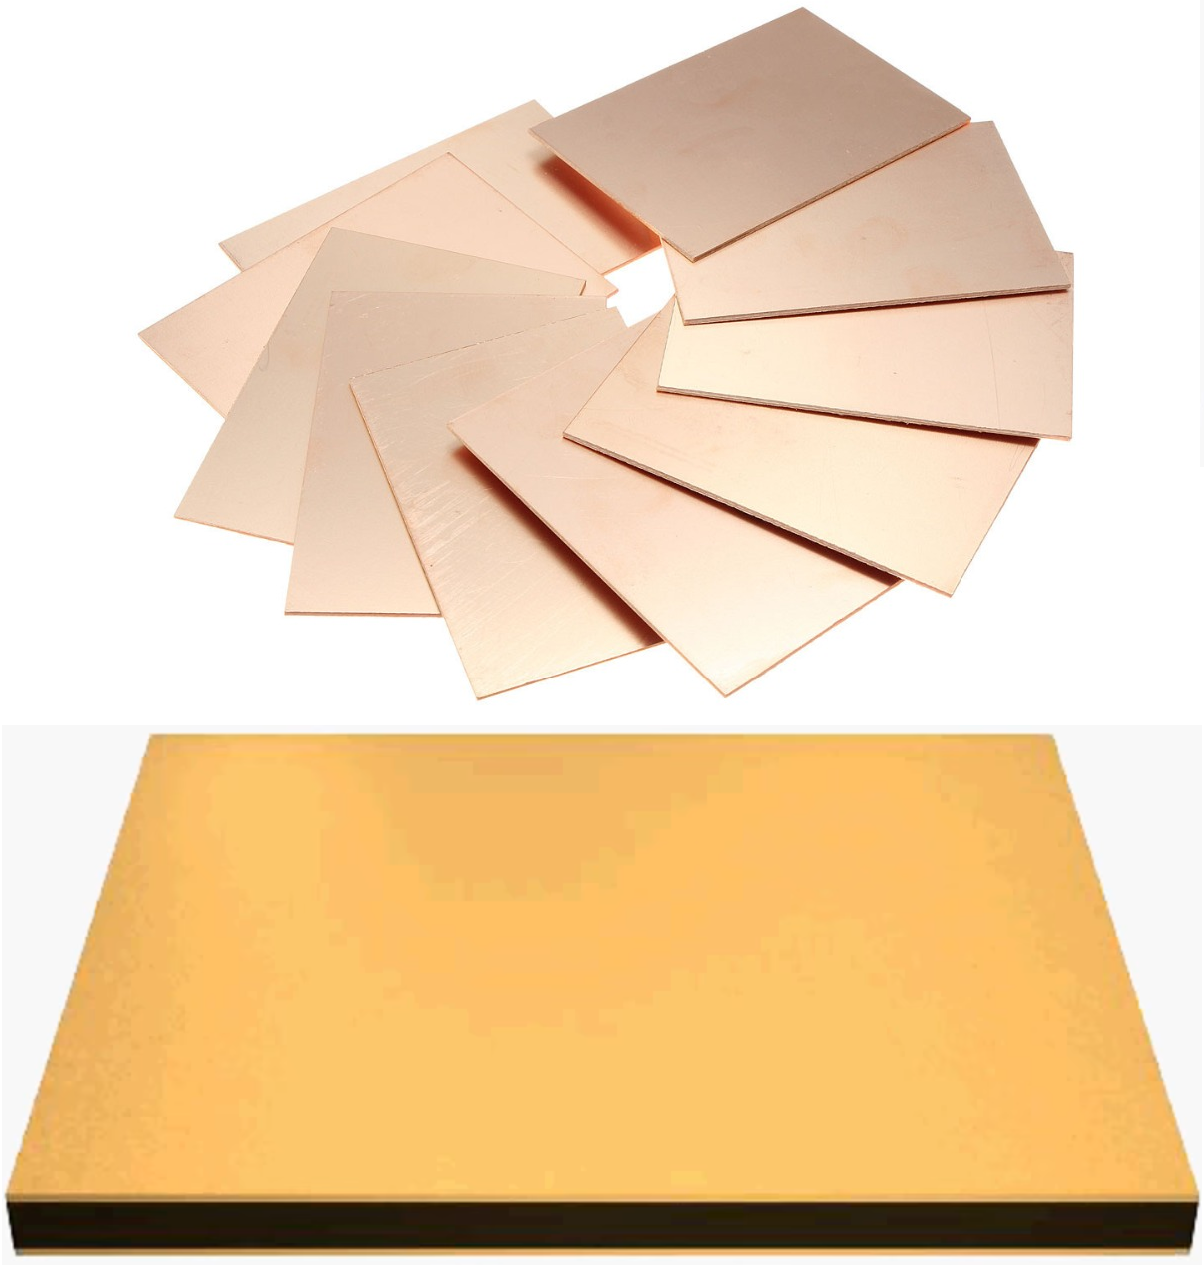
\includegraphics[scale=0.12]{jadro.png} & \textbf{Základ sendvičové struktury:}
			\begin{itemize}
				\item jádro izolantu FR4 s Cu vrstvami po oubou stranách,
				\item vrstvy jsou napařovány a pryskyřice je vytvrzována při specifickém tlaku (od $1.9$~MPa do $2.8$~MPa) a teplotě (kolem 190~$^\circ$C),
			\end{itemize}
			\end{tabular}
		\end{center}
		
		\begin{itemize}
			\item Jádro je základem i pro vícevrstvé plošné spoje a tvoří významnou část z celkové toušťky výsledného plošného spoje.
		\end{itemize}
	
\end{frame}
%------------------------------------------------------------------------------
\begin{frame}
	\frametitle{Vrtání děr do jádra}

	\begin{center}
		\begin{tabular}{m{0.5\linewidth} m{0.4\linewidth}}
		\textbf{Jádro se vrtá jen:}
		\begin{itemize}
			\item dvoustranném plošném spoji nebo
			\item pokud existují prokovy, které nejsou průchozí do krajních vrstev..
		\end{itemize}
		 & 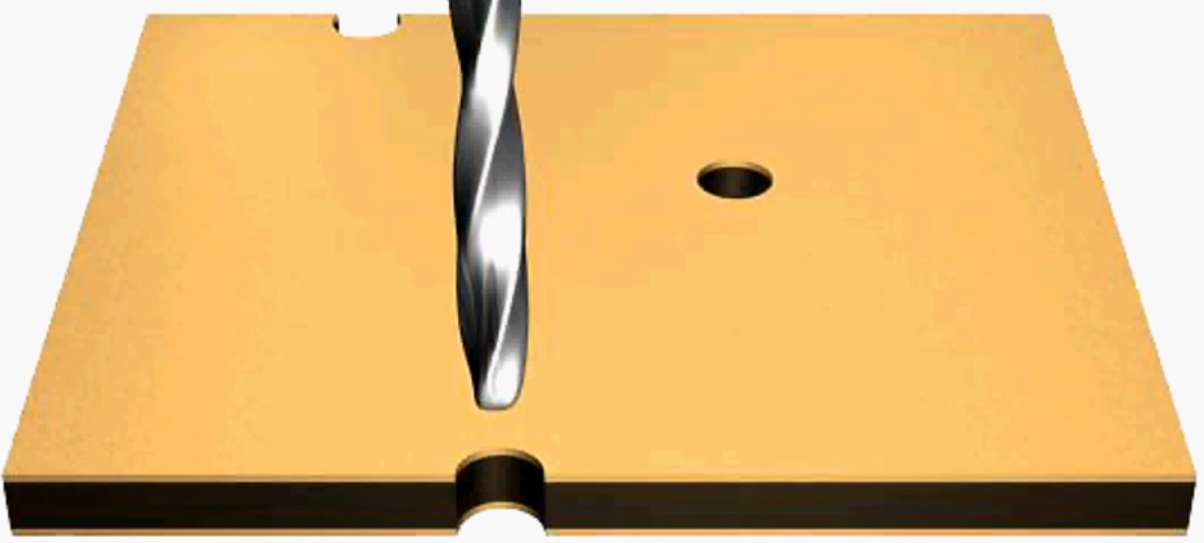
\includegraphics[scale=0.12]{jadroVrtani.png}
		\end{tabular}
	\end{center}
	
	K propojení obou stran dochází pomocí prokovených děr.
	\begin{center}
	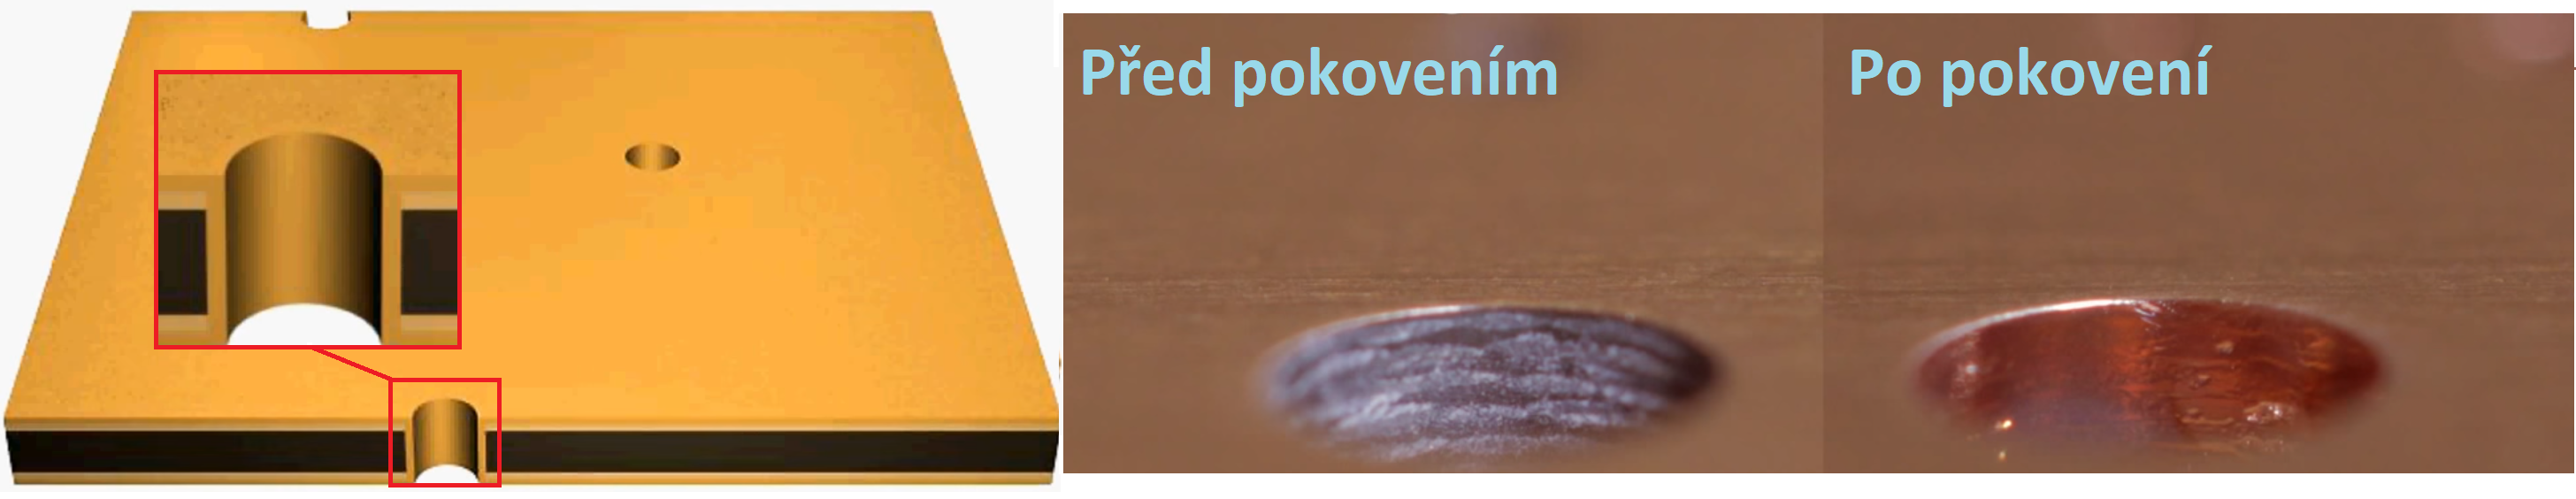
\includegraphics[scale=0.14]{jadroProkovy.png}
	\end{center}
\end{frame}
%------------------------------------------------------------------------------
\begin{frame}
	\frametitle{Nanášení fotorezistu}

	\begin{flushleft}
		\begin{tabular}{m{0.5\linewidth} m{0.4\linewidth}}
		\begin{itemize}
			\item fotorezist se aplikuje tlakem při zvýšené teplotě,
			\item nejčastěji se nanáší válcováním,
			\item v malosériových výrobách může být nanášen stříkáním (amatérská výroba),
			\item nanesená vrstva je velmi citlivá na UV záření,
		\end{itemize}
		 & 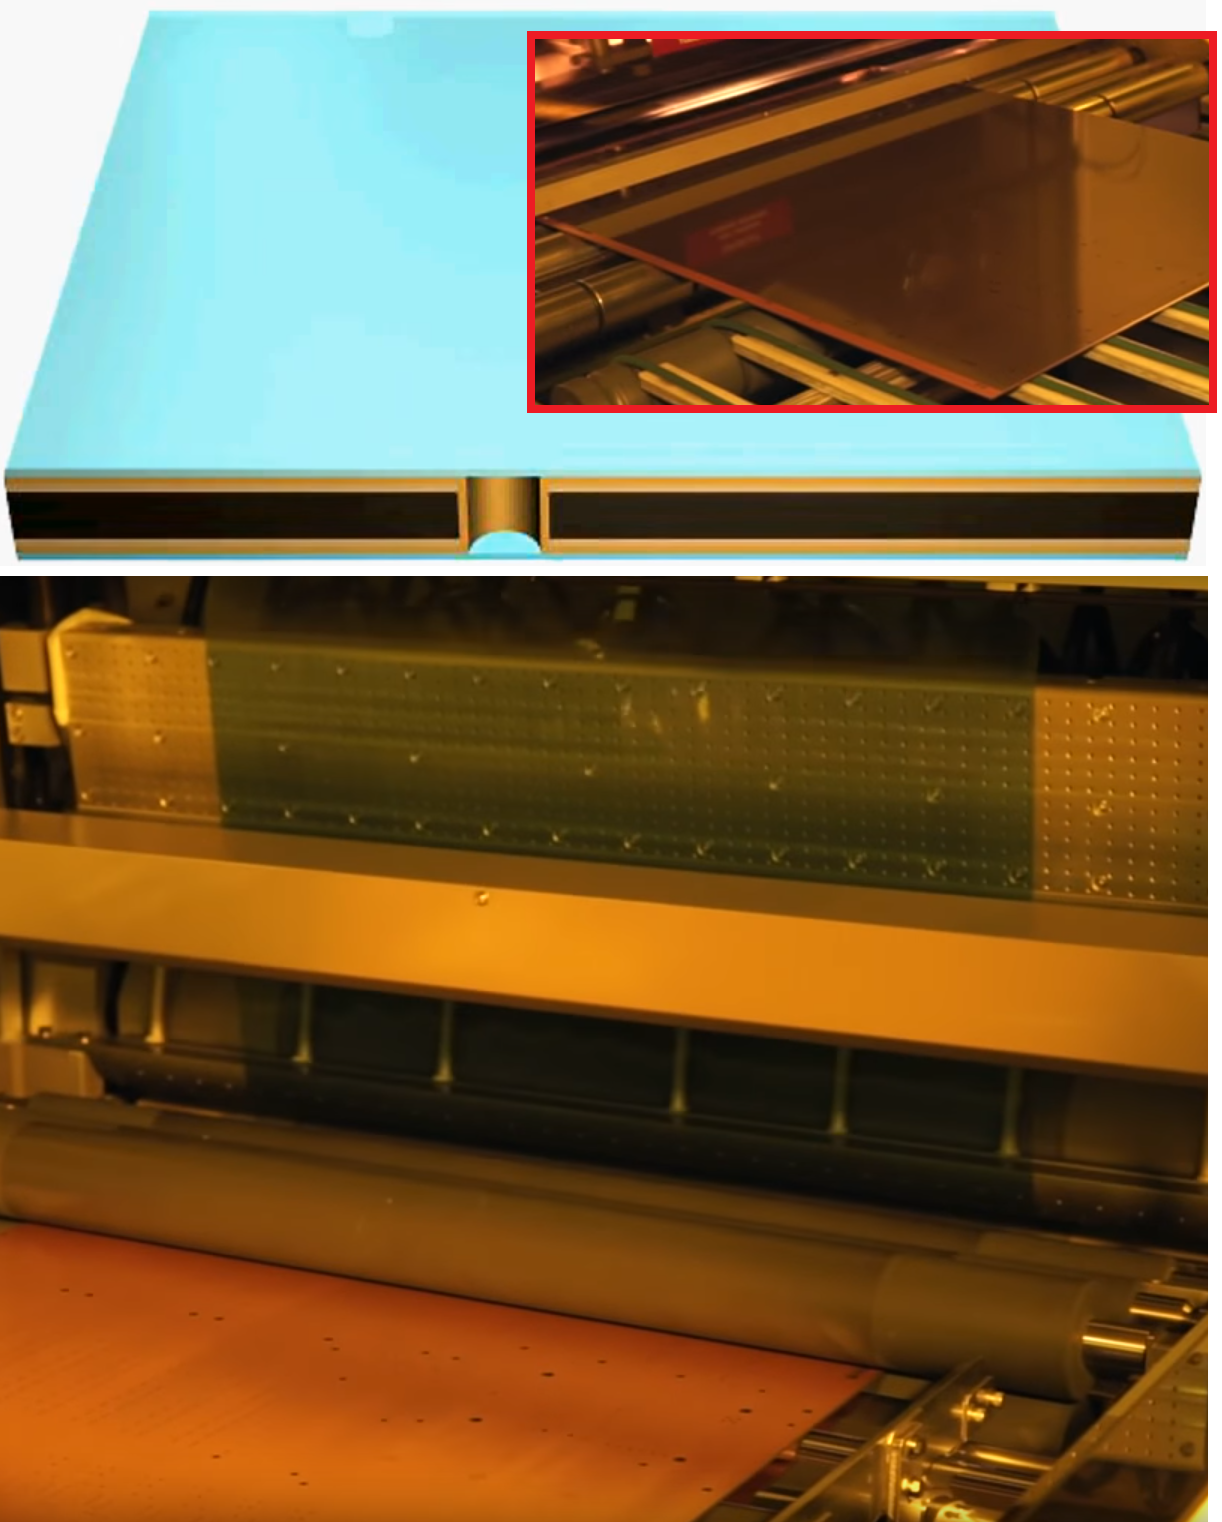
\includegraphics[scale=0.12]{jadroFotofilm.png}
		\end{tabular}
		\begin{tabular}{m{0.9\linewidth}}
		\begin{itemize}
			\item v prostorách zpracovávajících fotorezist se používá světlo s dlouhou vlnovou délkou (červené), aby bylo zabráněno předčasné expozici.
		\end{itemize}
		\end{tabular}
	\end{flushleft}

\end{frame}
%------------------------------------------------------------------------------
\begin{frame}
	\frametitle{Typy fotorezistů}

	\begin{center}
		\begin{tabular}{m{0.35\linewidth} m{0.55\linewidth}}
		 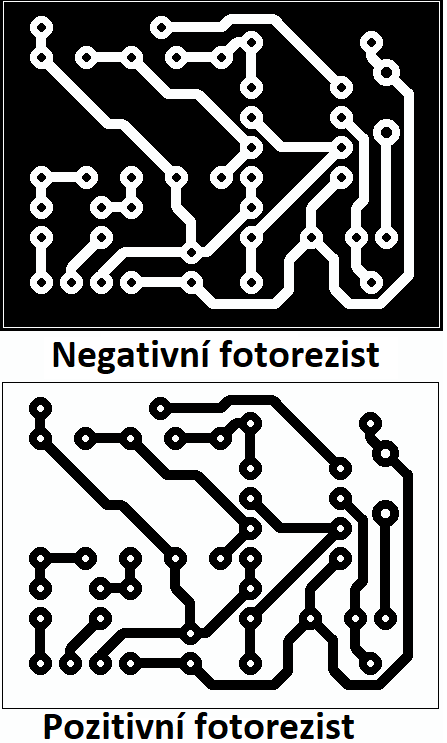
\includegraphics[width=0.3\textwidth]{negativAPozitiv.png} &
			Jsou možné dvě reakce fotorezistu na expozici:
			
			\begin{enumerate}
				\item exponované prostory polymerizují nebo
				\item jsou chemicky narušeny a je je možné rozpustit ve vyvolávací lázni.
			\end{enumerate}
			V prvním případě se jedná o negativní fotorezist, jelikož je žádaná chybějící část masky. Druhý je pozitivní fotorezist. V hromadné výrobě se obvykle využívá negativní fotorezist. 
		\end{tabular}
	\end{center}
	
\end{frame}
%------------------------------------------------------------------------------
\begin{frame}
	\frametitle{Expozice a vyvolání}

	\begin{center}
		\begin{tabular}{m{0.35\linewidth} m{0.55\linewidth}}
		 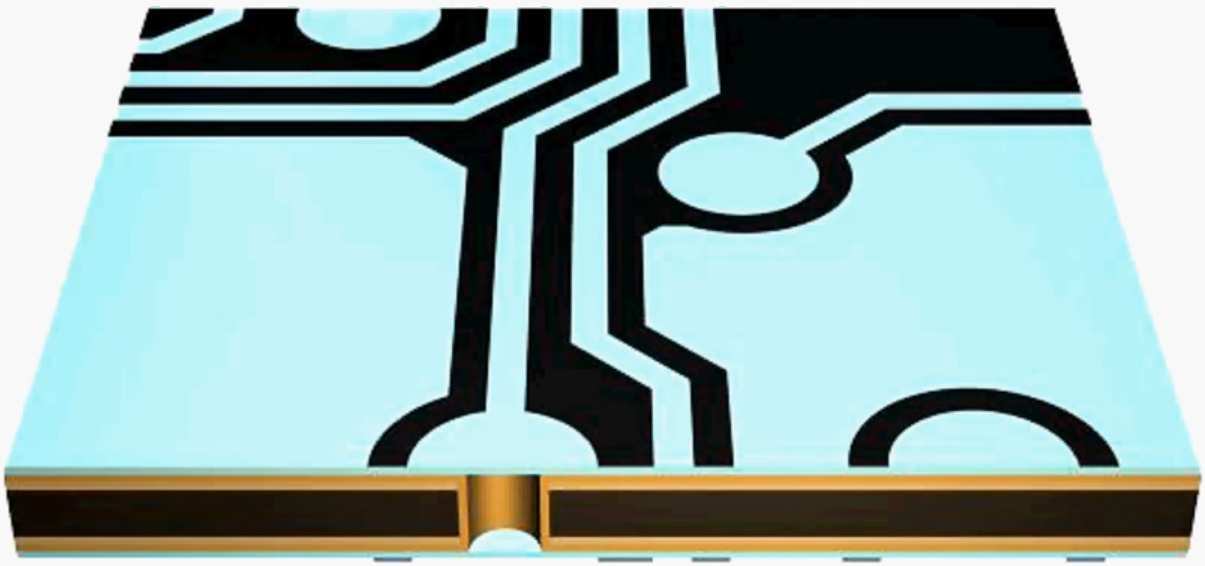
\includegraphics[scale=0.12]{jadroOsvit.png} &
			
			\begin{itemize}
				\item[$\Leftarrow$] Desky se exponují v UV světle,
				\item[$\Downarrow$] po odstranění nežádoucí vrstvy rezistu, zůstává v každém případě obrazec plošného spoje.
			\end{itemize}
		\end{tabular}
		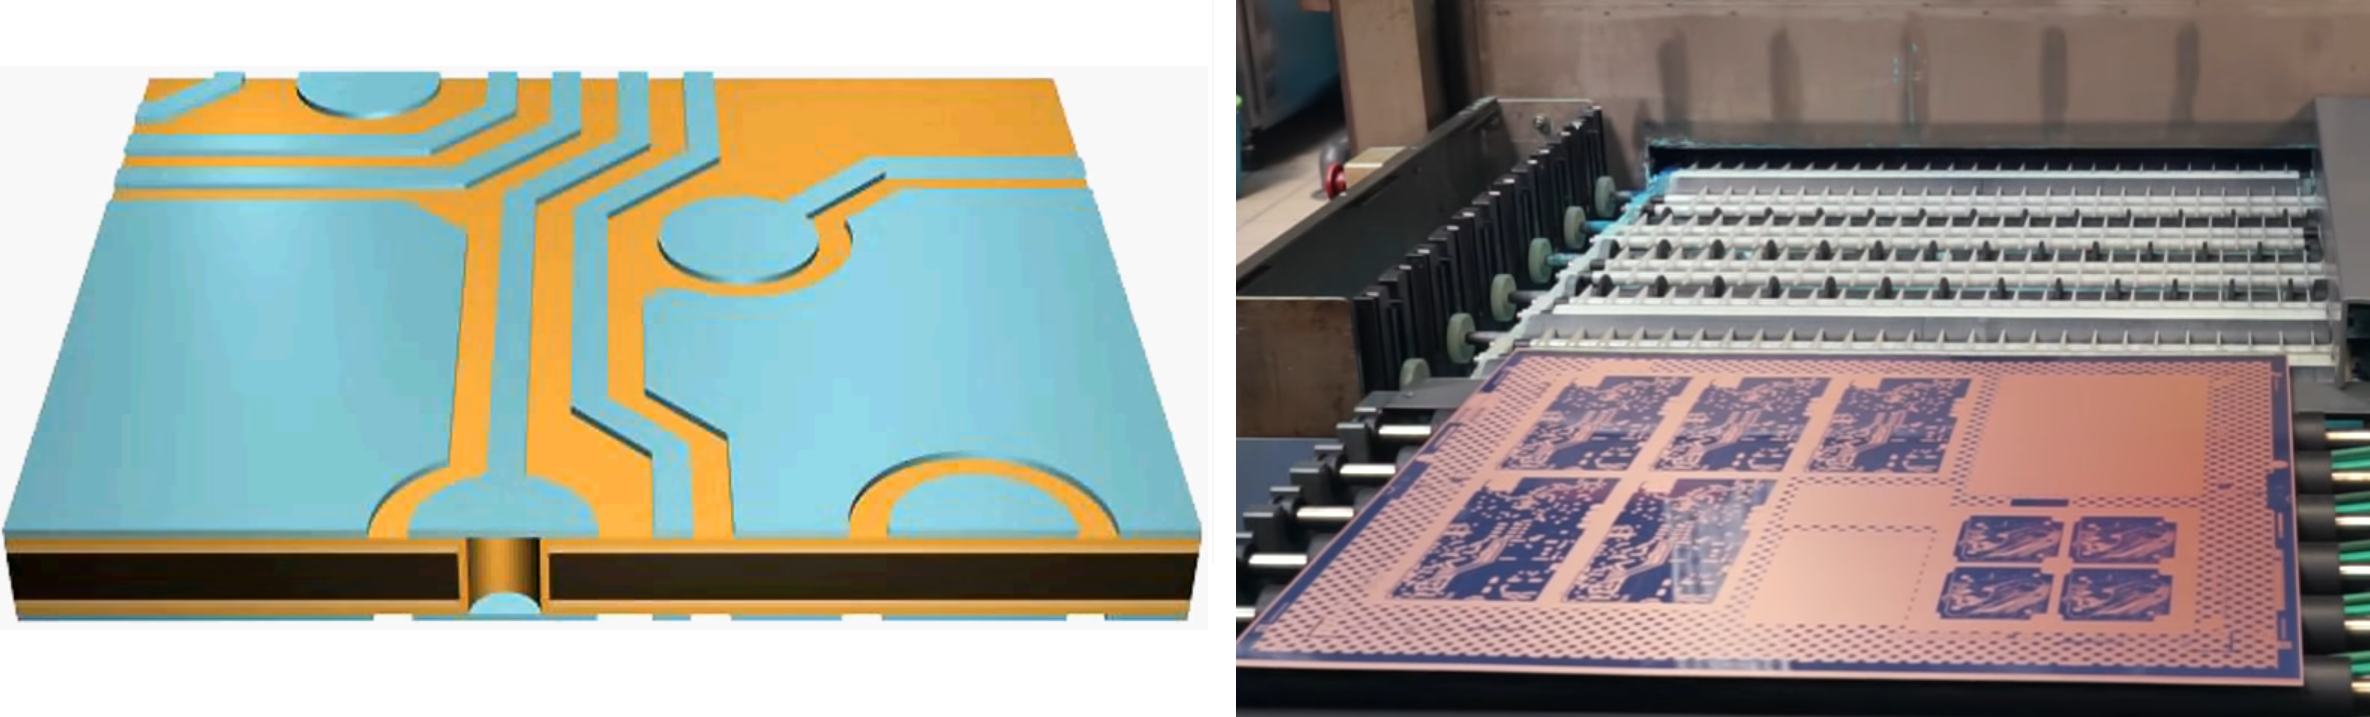
\includegraphics[scale=0.15]{jadroVyvolani.png}
	\end{center}
	
\end{frame}
%------------------------------------------------------------------------------
\begin{frame}
	\frametitle{Leptání}

	\begin{center}
		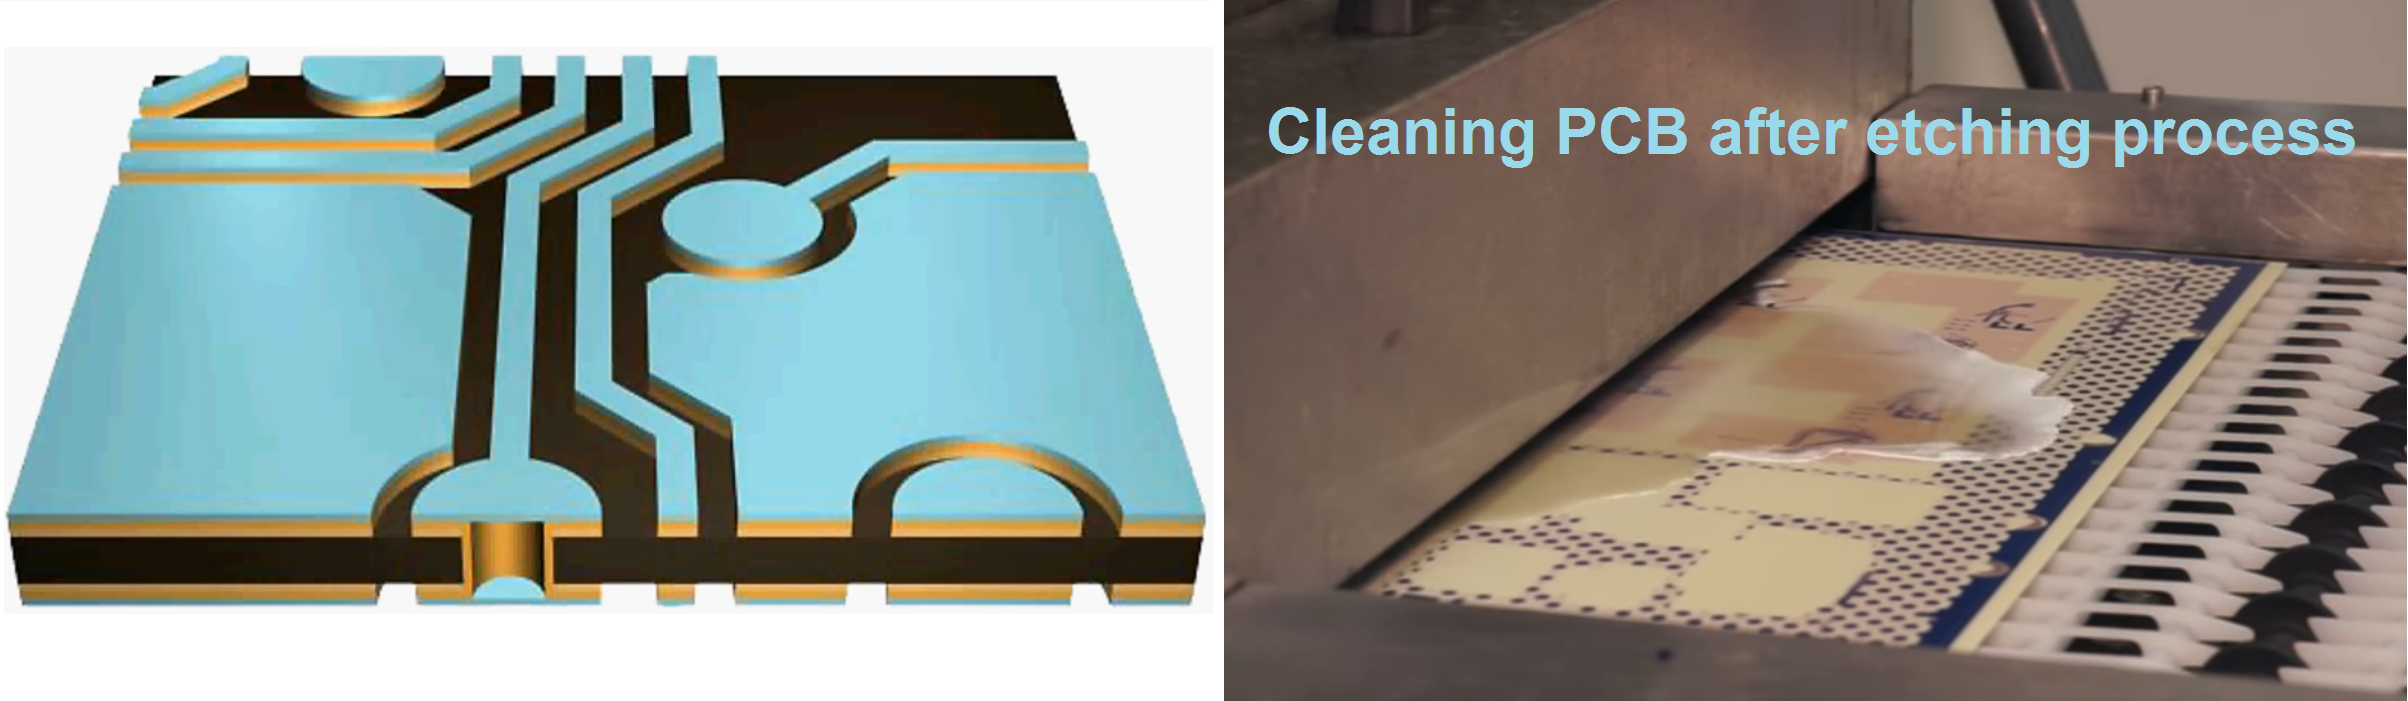
\includegraphics[scale=0.15]{jadroLeptani.png}
	\end{center}
	
	\begin{itemize}
		\item Pokud jsou v jádře otvory, pak jsou zamaskovány rezistem.
		\item Měď, která není chráněna rezistem, je rozpuštěna v kyselině.
		\item Obvyklé lázně jsou založené na chloridu měďnatém, chloridu železitém.
	\end{itemize}
\end{frame}
%------------------------------------------------------------------------------
\begin{frame}
	\frametitle{Dokončení jádra DPS}

	\begin{center}
		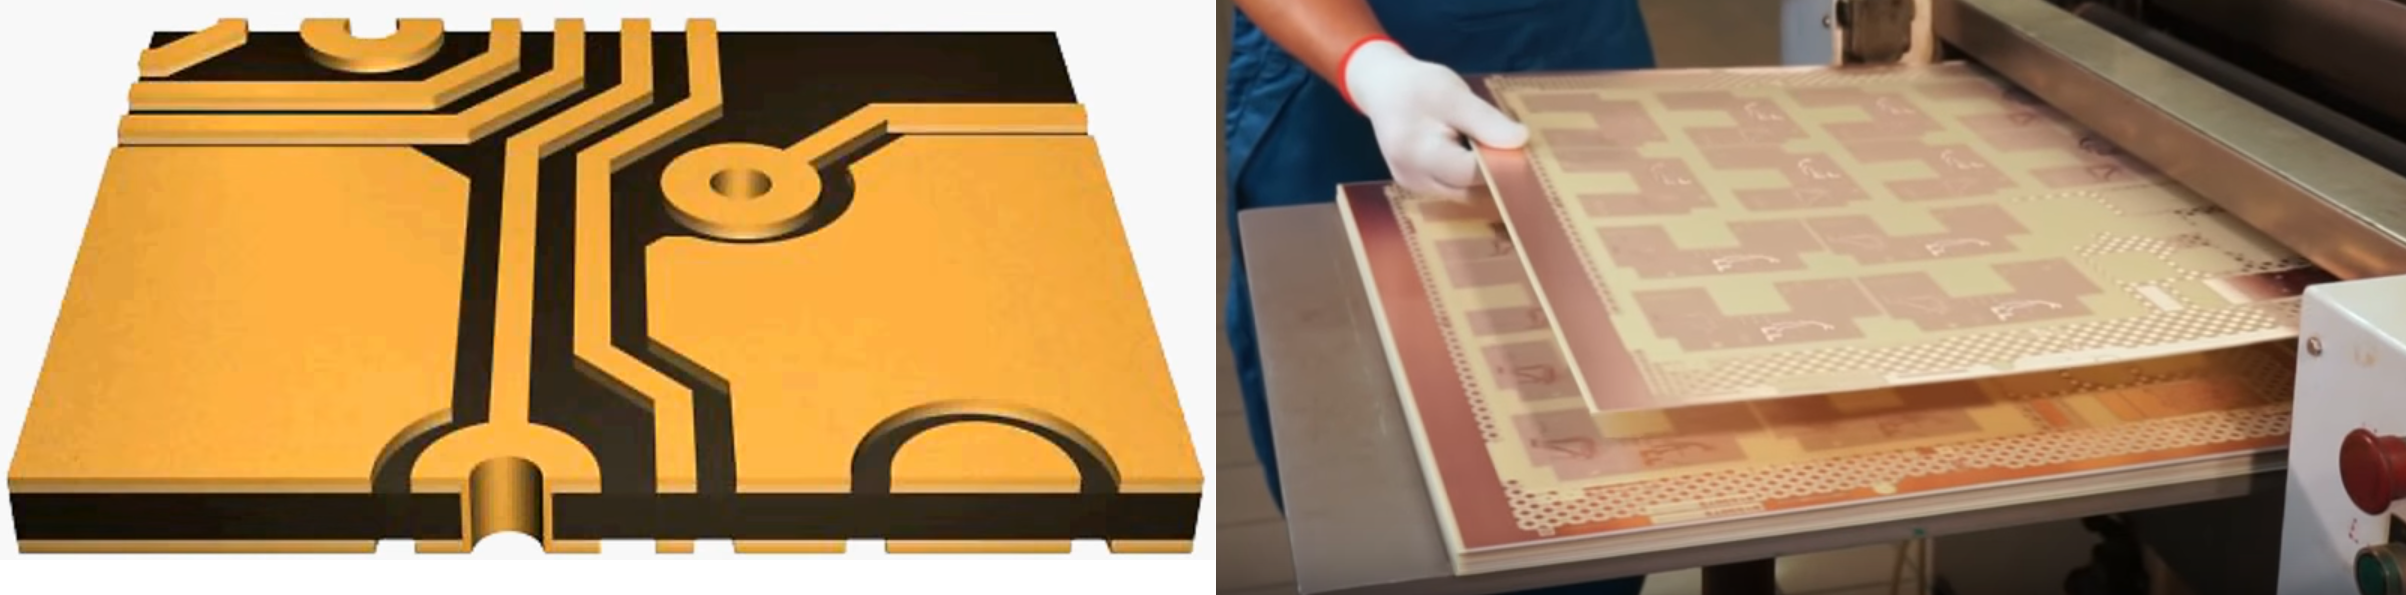
\includegraphics[scale=0.15]{jadroHotovo.png}
	\end{center}
	
	\begin{itemize}
		\item Po dokončení je jádro umyto a spoje procházejí automatickou optickou inspekcí.
		\item Pokud se jedná jen o dvouvrstvý spoj, pak proces pokračuje depozicí nepájivé masky.
		\item Při vícevrstvém spoji následuje proces tvorby dalších vrstev.
	\end{itemize}
\end{frame}

%------------------------------------------------------------------------------
\section{\texorpdfstring{Přidávání dalších vrstev}{Pridavani dalsich vrstev}}
%------------------------------------------------------------------------------

\begin{frame}
	\frametitle{Zakládání vrstev}

	\begin{center}
		\includegraphics[scale=0.10]{Platovani.png}
	\end{center}
	\begin{flushleft}
		\textbf{Ručně se přidávají další vrstvy:}
	\end{flushleft}
	\begin{center}
		\begin{tabular}{p{0.45\linewidth} p{0.45\linewidth}}
		
		\begin{enumerate}
			\setcounter{enumi}{0}
			\item Do spod se vkládá Cu a prepreg vrstva,
			\item vložení jádra,
		\end{enumerate}
		&
		\begin{enumerate}
			\setcounter{enumi}{2}
			\item vložení vrchní prepreg vrstvy,
			\item vložení vrchní Cu vrstvy.
		\end{enumerate}
		\end{tabular}
		\small
		\textbf{prepreg} je nevytvrzená vrstva FR4.
	\end{center}
\end{frame}
%------------------------------------------------------------------------------
\begin{frame}
	\frametitle{Porovnání tlouštěk vrstev - zdroj Pragoboard}

	\begin{center}
		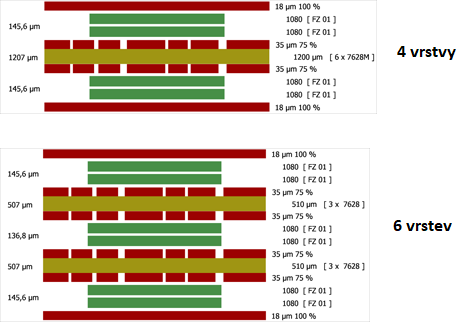
\includegraphics[scale=0.8]{pragoboard.png}
	\end{center}
	
	
	\begin{itemize}
		\item DPS může obsahovat více jader,
		\item některé vrstvy mají menší izolační vzdálenost.
	\end{itemize}
	
\end{frame}
%------------------------------------------------------------------------------
\begin{frame}
	\frametitle{Slepení vrstev pomocí tlaku a tepla}

	\begin{center}
		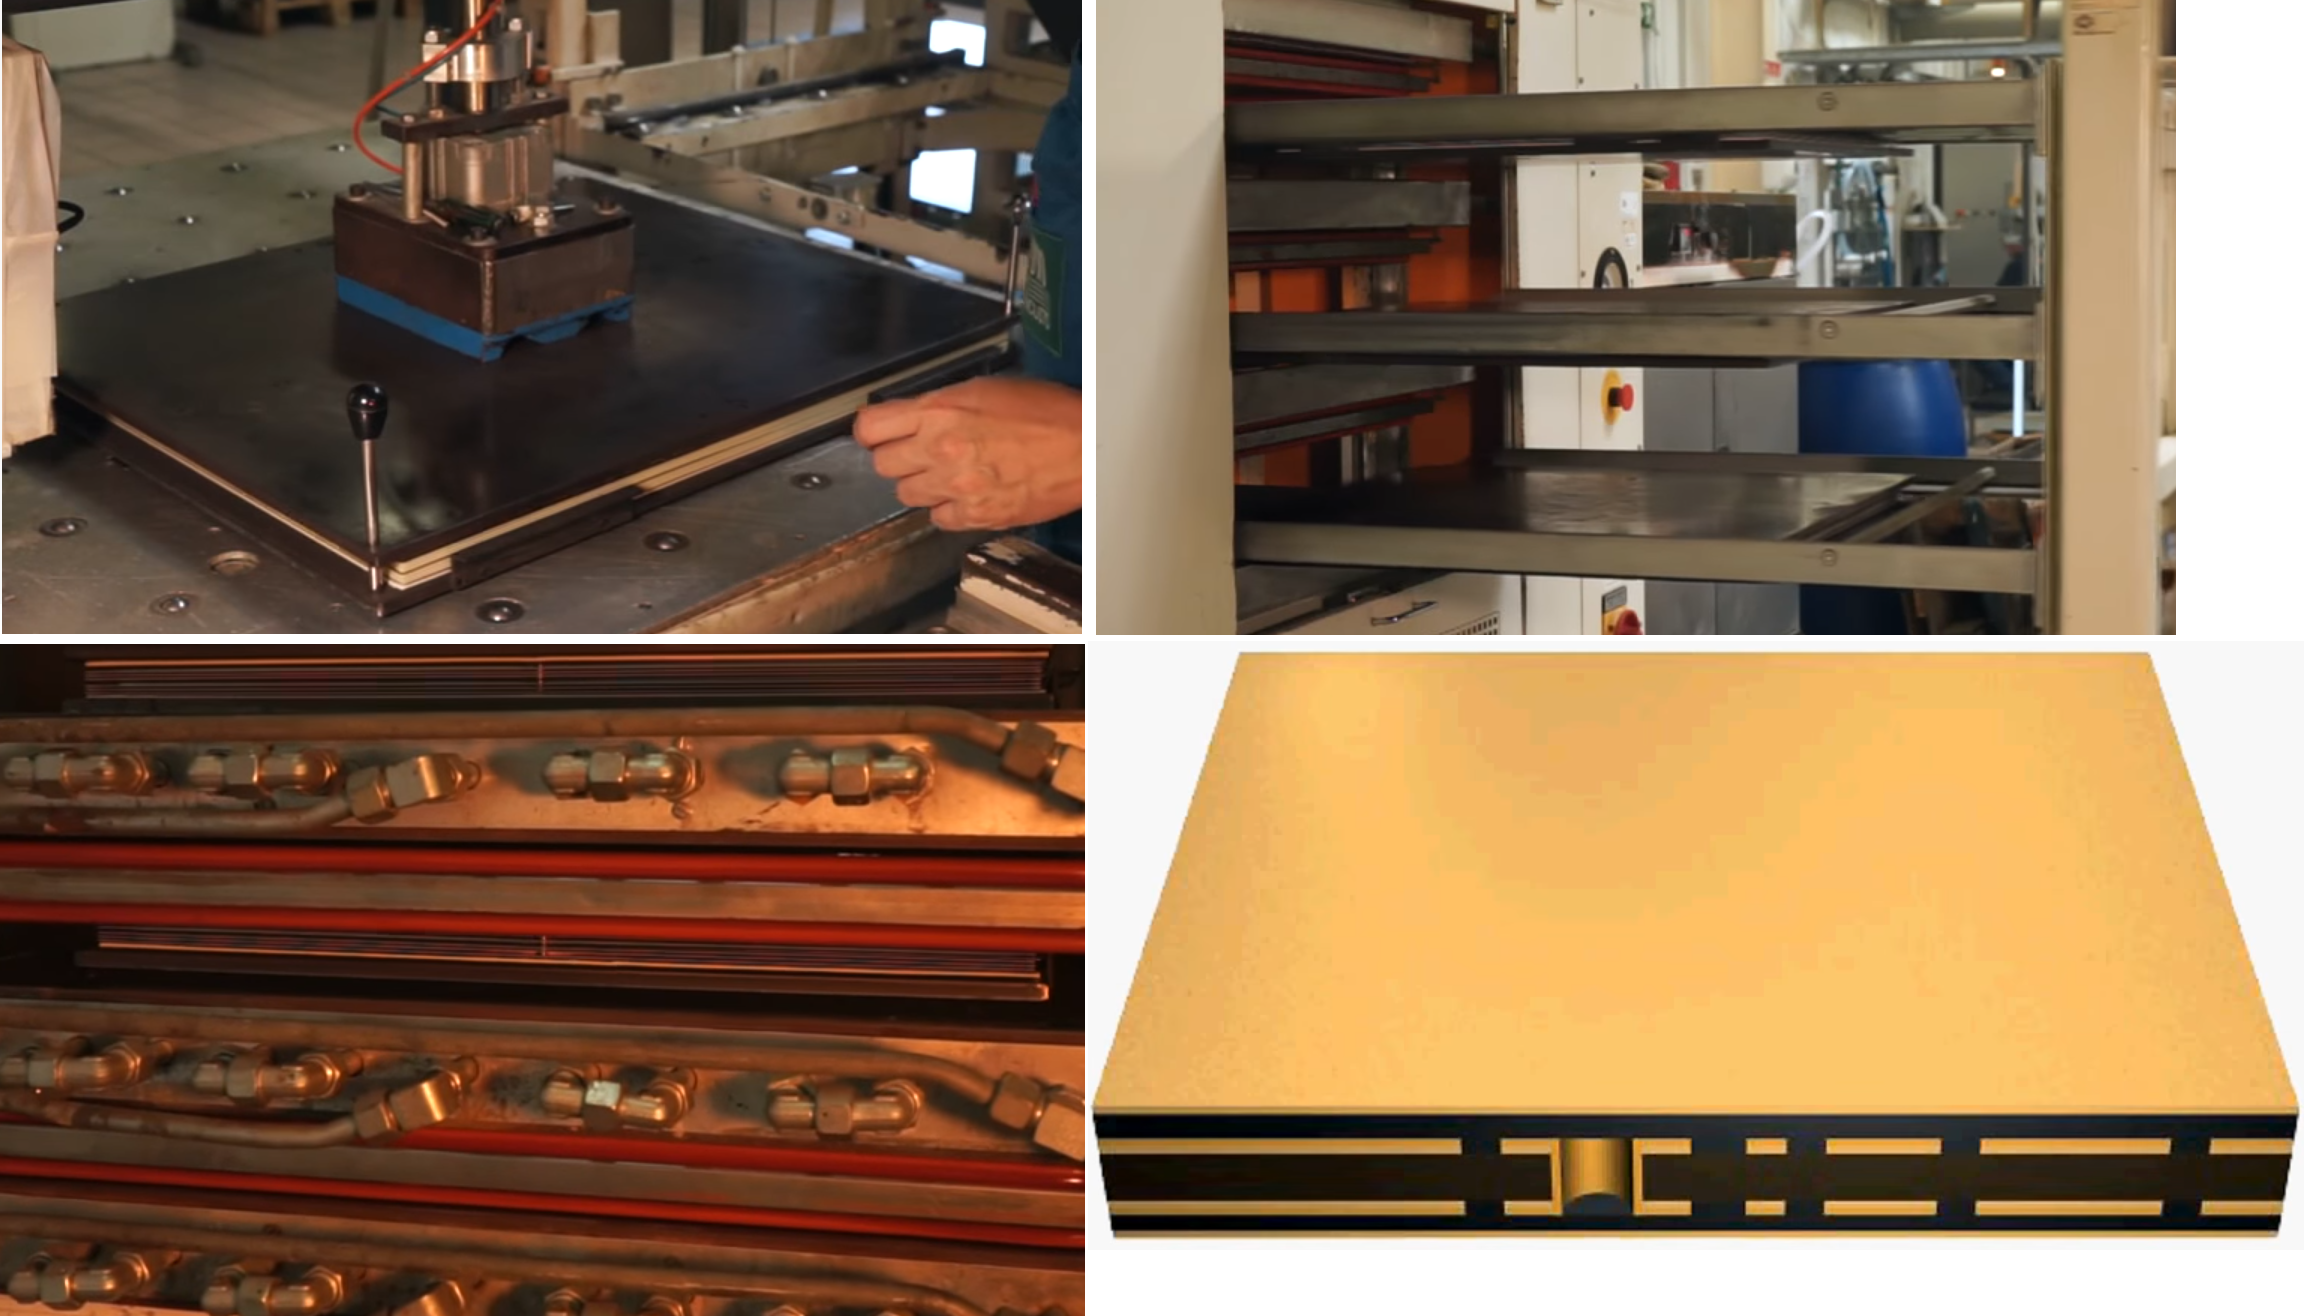
\includegraphics[scale=0.15]{vnejsiCuFilm.png}
	\end{center}
	
	\begin{itemize}
		\item Používá se podobný proces jako při laminaci jádra. Pryskyřice se vytvrzuje při teplotách okolo $190$~$^\circ$C.
	\end{itemize}
\end{frame}
%------------------------------------------------------------------------------
\begin{frame}
	\frametitle{Vrtání}

	\begin{center}
		\begin{tabular}{m{0.45\linewidth} m{0.45\linewidth}}
		 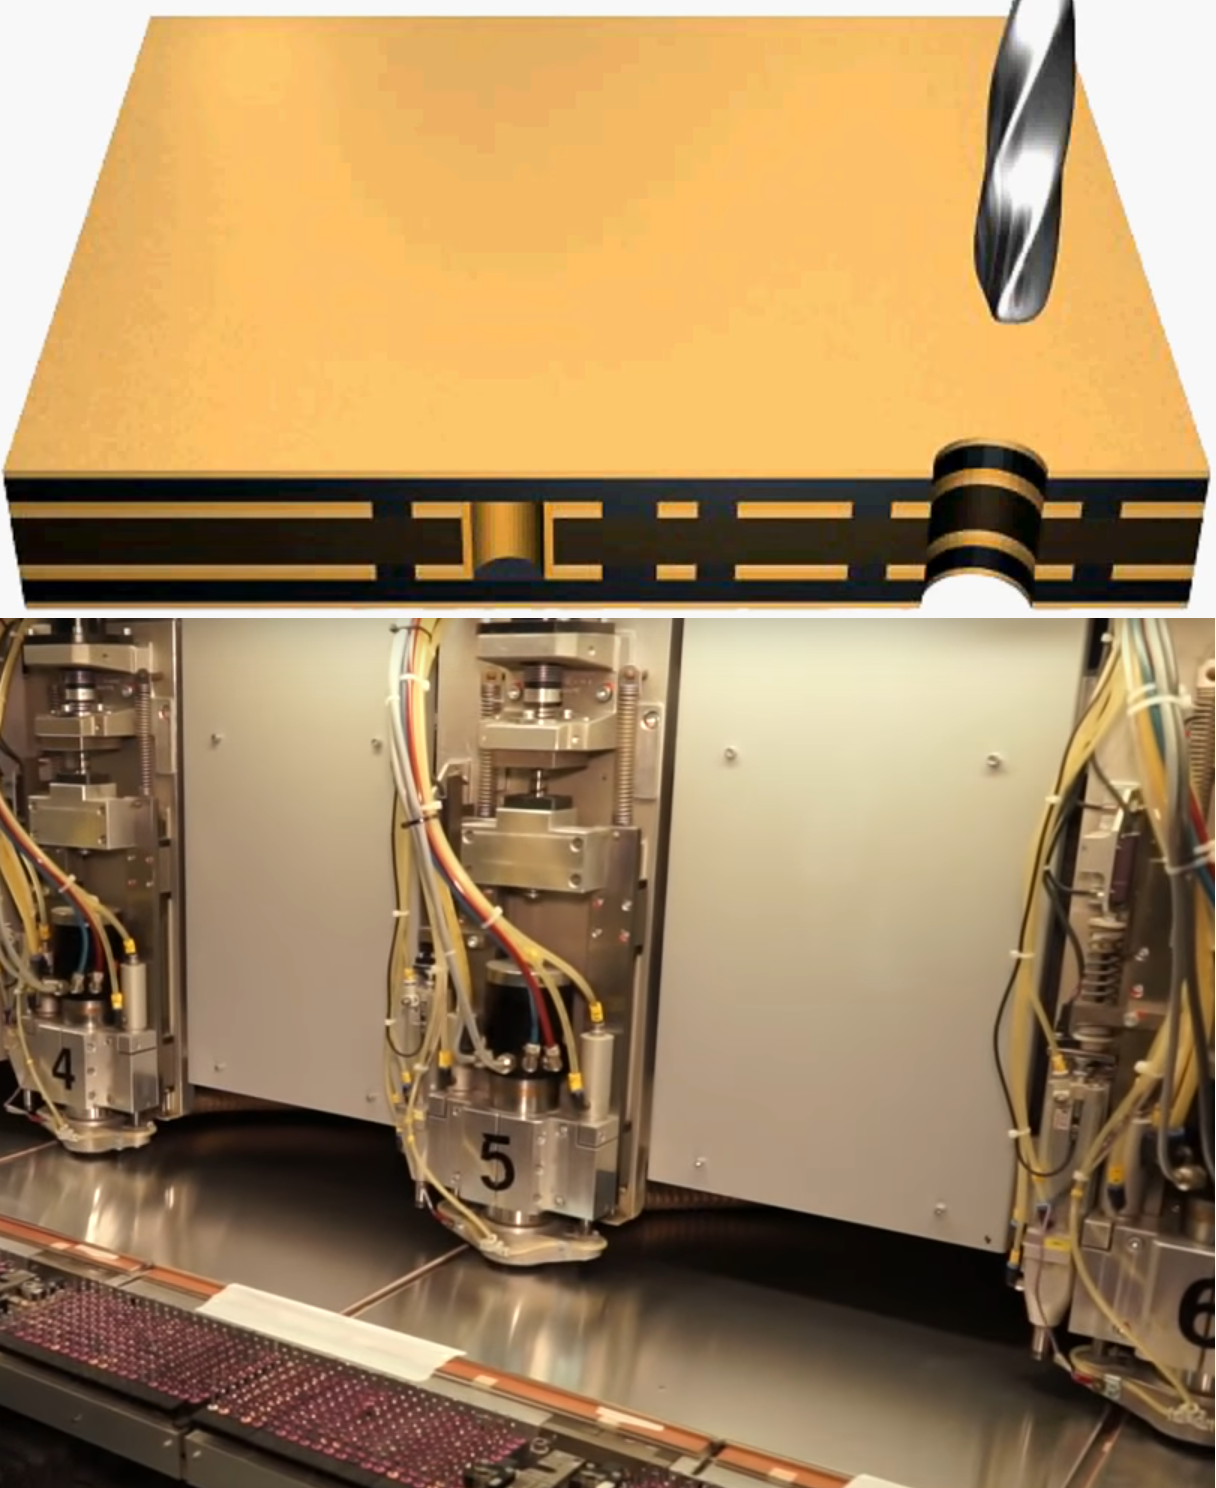
\includegraphics[scale=0.15]{vnejsiVrtani.png} &
			
			\begin{itemize}
				\item Více desek je vždy vrtáno najednou.
				\item Následuje prokovávání děr, podobně jako tomu bylo u realizace jádra.
			\end{itemize}
		\end{tabular}
	\end{center}
\end{frame}
%------------------------------------------------------------------------------
\begin{frame}
	\frametitle{Zpracování obrazce}
	...je to stejné jako u jádra:
	\begin{center}
	
		\begin{tabular}{m{0.05\linewidth} m{0.38\linewidth} m{0.05\linewidth} m{0.38\linewidth}}
		 \Large & 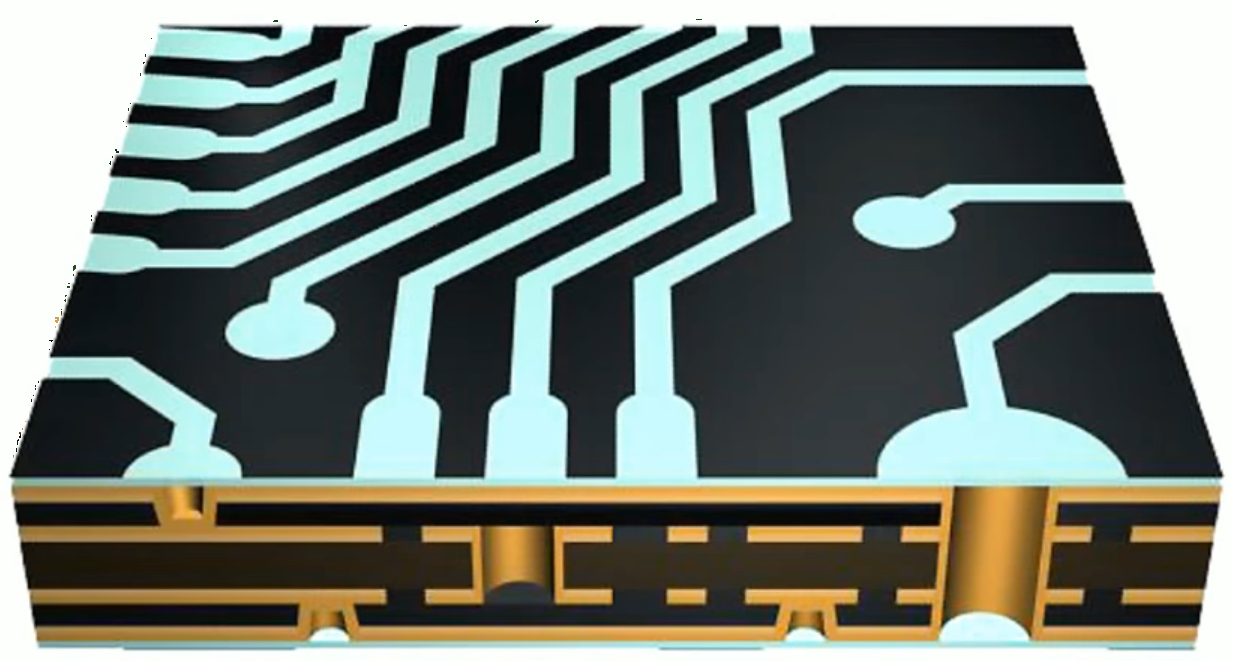
\includegraphics[scale=0.12]{vnejsiOsvit.png} & \Large\textbf{$\rightarrow$} & 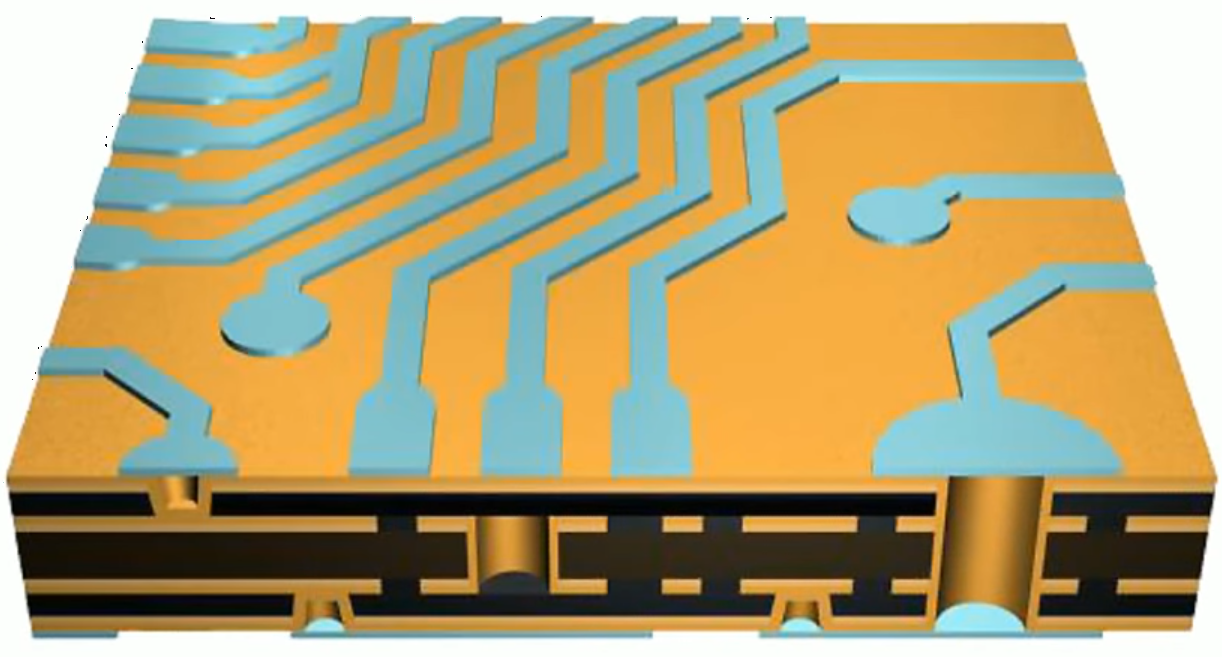
\includegraphics[scale=0.12]{vnejsiVyvolani.png}\\
		 & Depozice rezistu a UV expozice & & Vyvíjení \\
		 \Large\textbf{$\hookrightarrow$} & 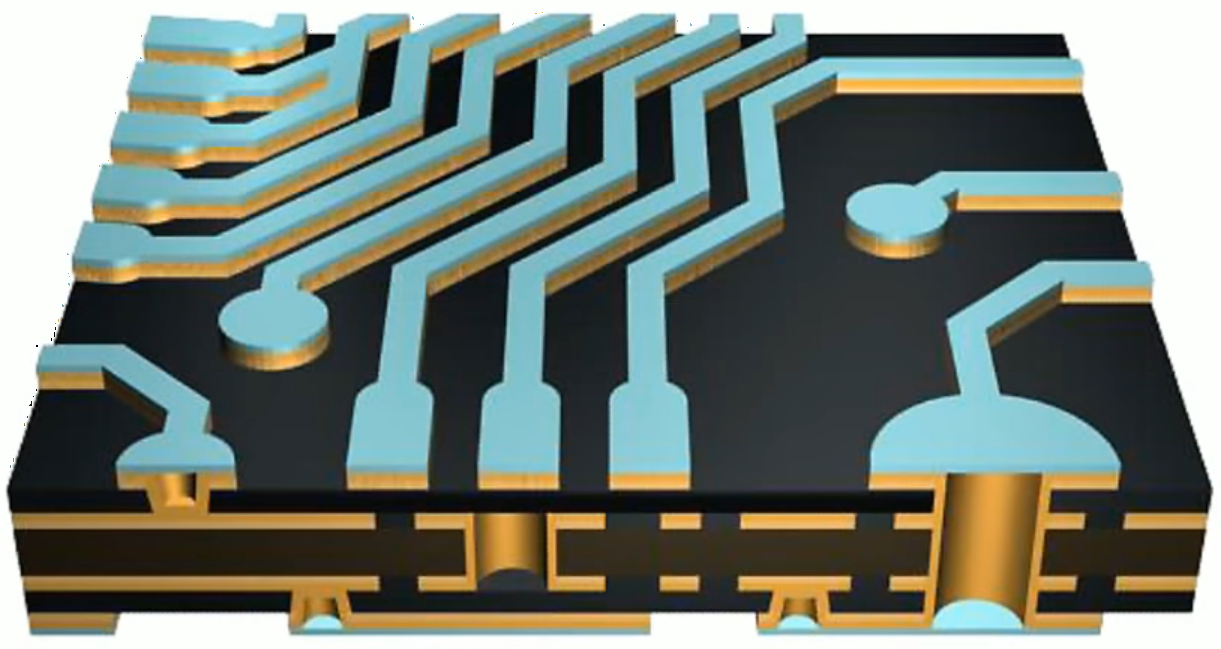
\includegraphics[scale=0.12]{vnejsiLeptani.png} & \Large\textbf{$\rightarrow$} & 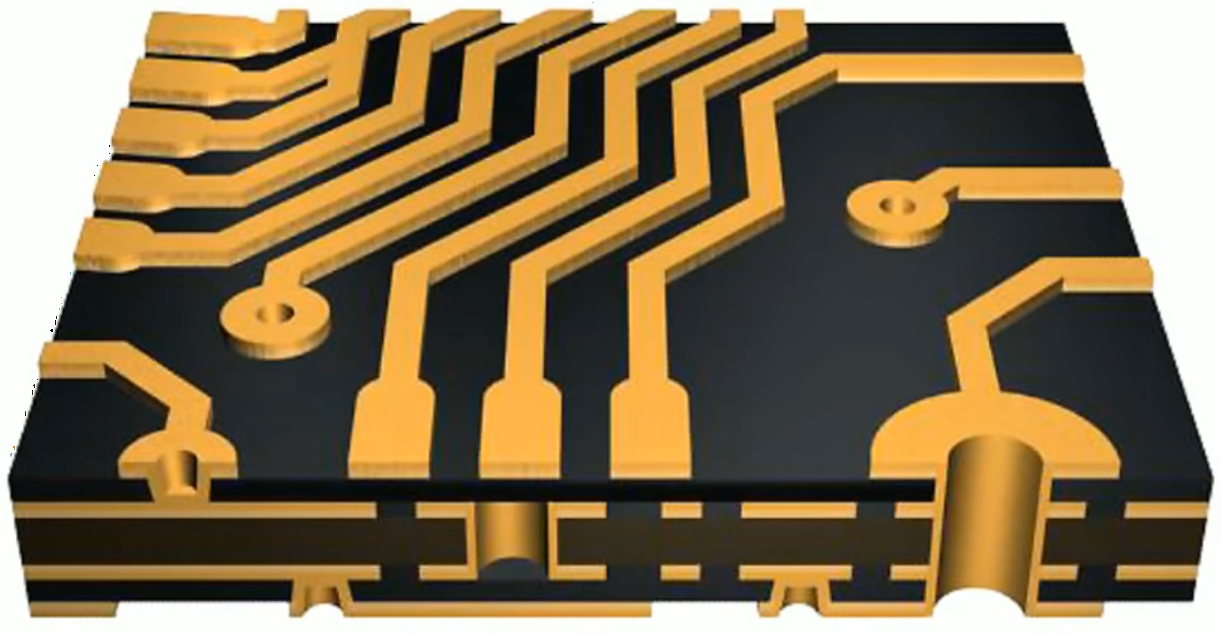
\includegraphics[scale=0.12]{vnejsiHotovo.png}\\
		& Leptání & & Mytí
		\end{tabular}
	\end{center}
\end{frame}
%------------------------------------------------------------------------------
\begin{frame}
	\frametitle{Tvorba nepájivé masky}
	...je téměř stejná jako fotolitografie:
	\begin{center}
	
		\begin{tabular}{m{0.05\linewidth} m{0.38\linewidth} m{0.05\linewidth} m{0.38\linewidth}}
		 \Large & \includegraphics[scale=0.12]{maskaFilm.png} & \Large\textbf{$\rightarrow$} & \includegraphics[scale=0.12]{maskaExpozice.png}\\
		 & Depozice masky & & Expozice \\
		 \Large\textbf{$\hookrightarrow$} & \includegraphics[scale=0.12]{maskaHotovo.png} & \Large\textbf{$\rightarrow$} & 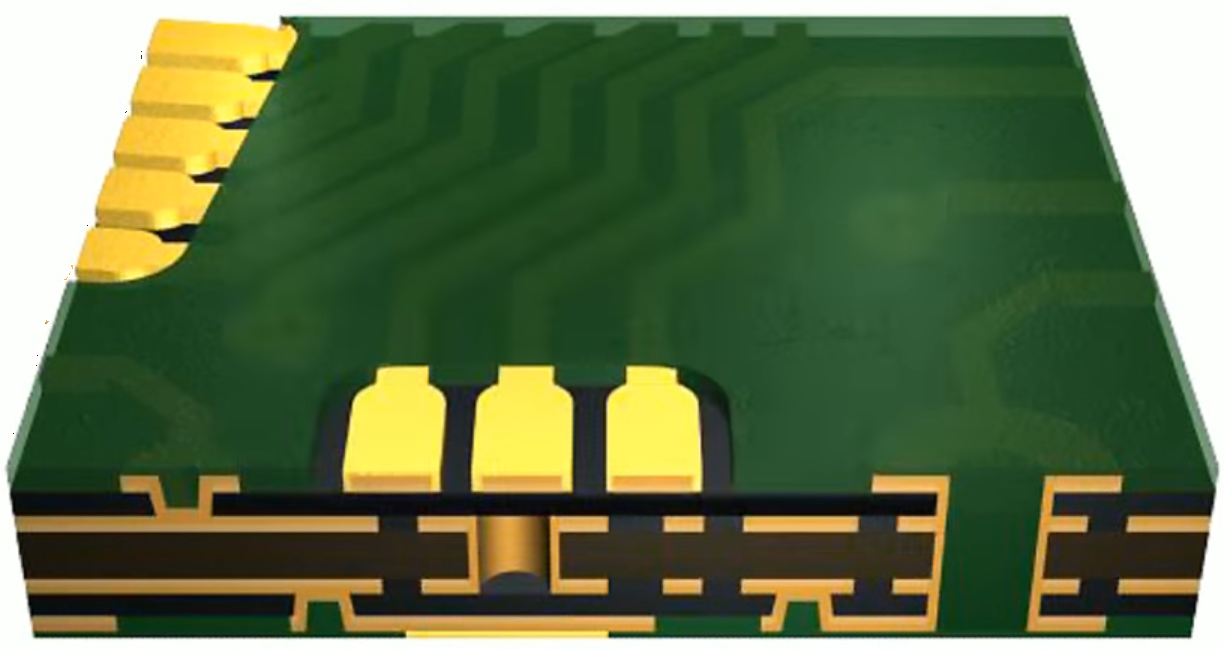
\includegraphics[scale=0.12]{Pokoveni.png}\\
		& Vyvíjení & & Pokovování
		\end{tabular}
	\end{center}
\end{frame}
%------------------------------------------------------------------------------
\begin{frame}
	\frametitle{Pokovování}

	\begin{center}
		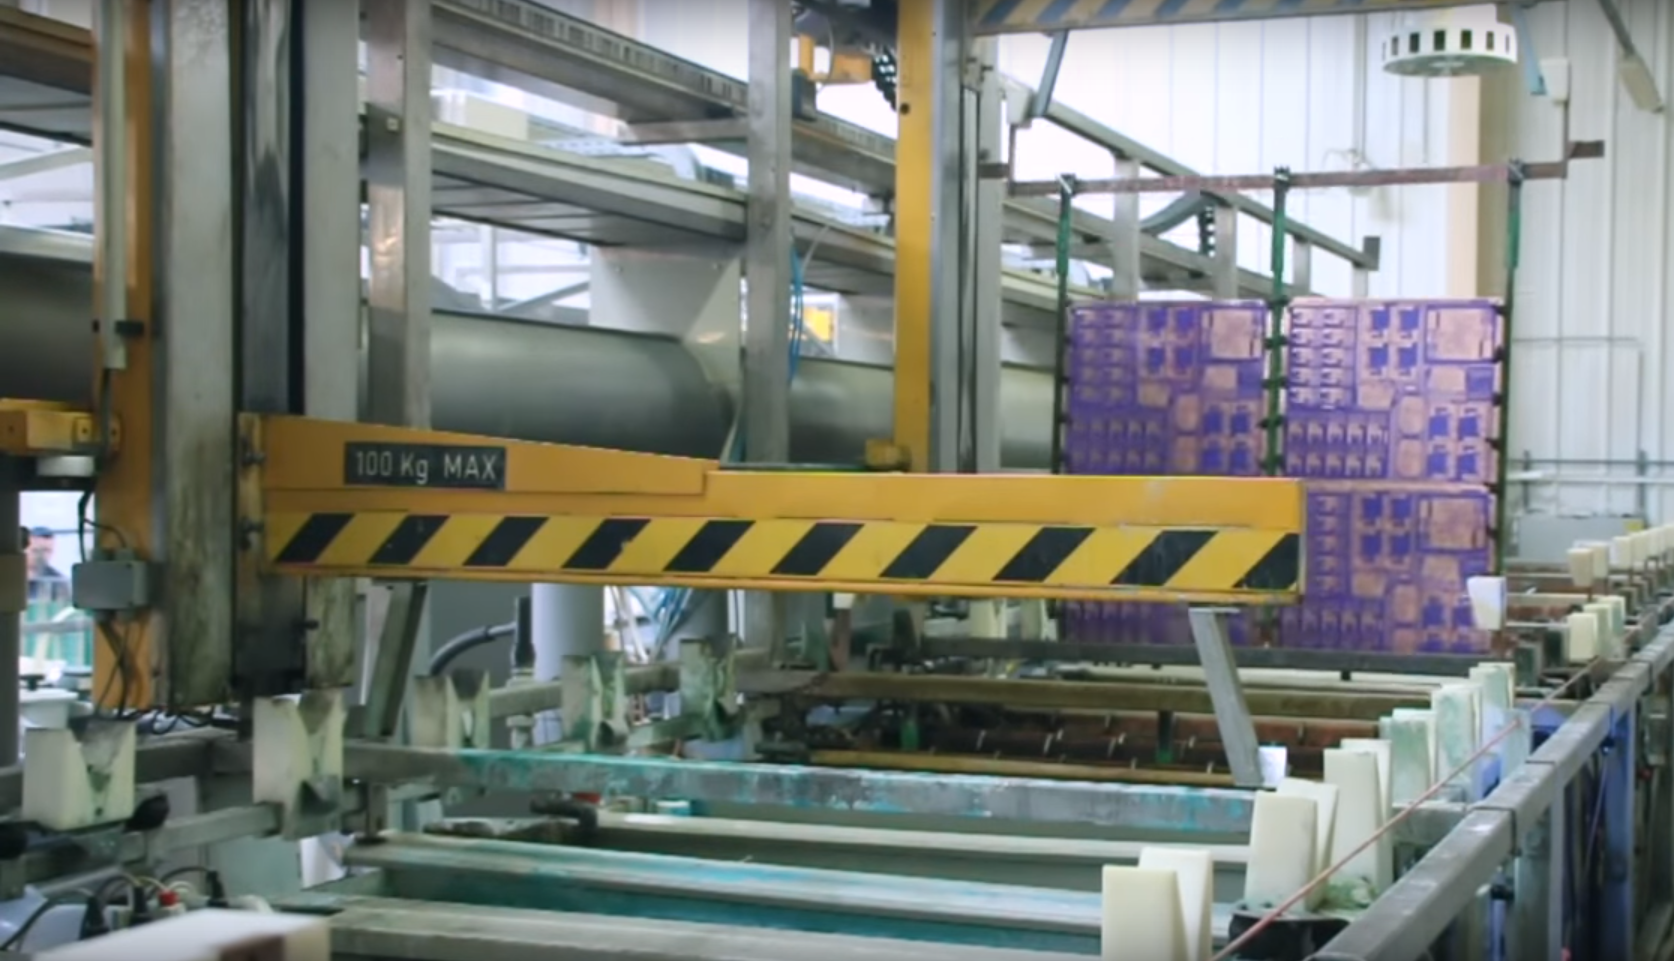
\includegraphics[scale=0.2]{procesProkovovani.png}
	\end{center}
	
\end{frame}

%------------------------------------------------------------------------------
\begin{frame}
	\frametitle{Jen orientační přehled možných pokovovacích procesů}

\begin{enumerate}
	\item \textbf{HASL} - žárové cínování, halovaní
	\begin{itemize}
		\item skvělá pájitelnost, levné,
		\item vrstvy vykazují nerovnosti, nehodí se pro SMD montáž $<20$~mil.
	\end{itemize}
	
  \item \textbf{ENIG} - imerzní zlacení
	
	\begin{itemize}
		\item rovnoměrné plochy, dobrá pájitelnost, vhodné pro drobné SMD a BGA,
		\item chemický proces může být agresivní vůči nepájivé masce, je to drahé
	\end{itemize}
	
	\item \textbf{Galvanické zlacení}
	\begin{itemize}
		\item rovnoměrné plochy, dobrá pájitelnost, otěruvzdorné a tudíž vhodné pro konektory,
		\item zlacené plošky musejí mít mezi sebou vodivý kontakt, je to drahé
	\end{itemize}
	
	\item \textbf{Imerzní cín}
	
	\begin{itemize}
		\item rovnoměrné plochy, dobrá pájitelnost,
		\item chemický proces může být agresivní vůči nepájivé masce, problém whiskerů
	\end{itemize}
	
\end{enumerate}
	
\end{frame}

%------------------------------------------------------------------------------
\section{\texorpdfstring{Technologická omezení}{Technologicka omezeni}}
%------------------------------------------------------------------------------
\begin{frame}
	\frametitle{Omezení plynoucí z principu výroby}

	\begin{itemize}
		\item U dvouvrstvé DPS musím počítat s izolační vzdáleností mezi oběma Cu vrstvami, která vždy zajistí dostatečnou mechanickou odolnost (obvyklé minimum je 0,4~mm).
		\item Nenavrhujeme lichý počet vodivých vrstev. Výjimkou je 1 vrstva. Při lichém počtu vrstev téměř jistě dojde k prohnutí DPS vlivem tepelného namáhání.
		\item U vícevrstvého plošného spoje mají vždy krajní vrstvy a nejbližší sousední vrstva nejmenší izolační vzdálenost (vhodné pro sledované vlastní impedance vedení).
		\item Vnitřní vrstvy je vhodné navrhovat celistvé (rozlitá měď). Cesty totiž mohou způsobovat nerovnosti v krajních vrstvách.
		\item Pokovení zvedne vertikální úroveň nezamaskovaných ploch (jde především o pady) a výrazně ovlivňuje osazování.
	\end{itemize}
\end{frame}
%------------------------------------------------------------------------------
\begin{frame}
	\frametitle{Omezení v závislosti na výrobci}

	\begin{itemize}
		\item Velmi často lze zvolit tloušťku Cu vnějších vrstev, ale vnitřní vrstvy mají tloušťku předepsanou.
		\item Volba tlouštěk Cu vrstev je omezena.
		\item Je nutné se seznámit s omezeními týkajících se minimální izolační mezery, šířky cest, průměrů otvorů atd.
		\item Pokud navrhujeme DPS se sledovanou vlastní impedancí, pak je obvyklé, že si volíte konkrétní materiál a necháváte si vyrobit kontrolní kupón.
		\item DPS je obvykle omezena minimální izolační vzdáleností vodivé cesty od okraje.
	\end{itemize}
\end{frame}
%------------------------------------------------------------------------------
\begin{frame}
	\frametitle{Omezení návrhu - vhodná skladba vrstev}

	\begin{itemize}
		\item 2 vrstvy: 
		
		\begin{itemize}
			\item \textbf{sig/pwr --core-- gnd}
		\end{itemize}
		
		\item 4 vrstvy: 
		
		\begin{enumerate}
			\item \textbf{sig -- gnd --core-- gnd -- sig/pwr},
			\item \textbf{sig -- gnd --core-- pwr -- sig}, 
			\item \textbf{sig -- gnd --core-- sig/pwr -- gnd}, 
		\end{enumerate}
		
		\textbf{ad 1.} rozvod napájení na spodní straně má výhodu snazšího vyvážení ploch,\\
		\textbf{ad 2.} občas problém s EMC, zpětné cesty proudů jdou přes pwr,\\
		\textbf{ad 3.} nutné vyvážit vnitřní vrstvu, nevhodné pro oboustrannou montáž.
	\end{itemize}
\end{frame}
%------------------------------------------------------------------------------
\begin{frame}
	\frametitle{Omezení návrhu - proudová zatížitelnost}
	
	\begin{center}
		\begin{tabular}{m{0.45\linewidth} m{0.45\linewidth}}
		 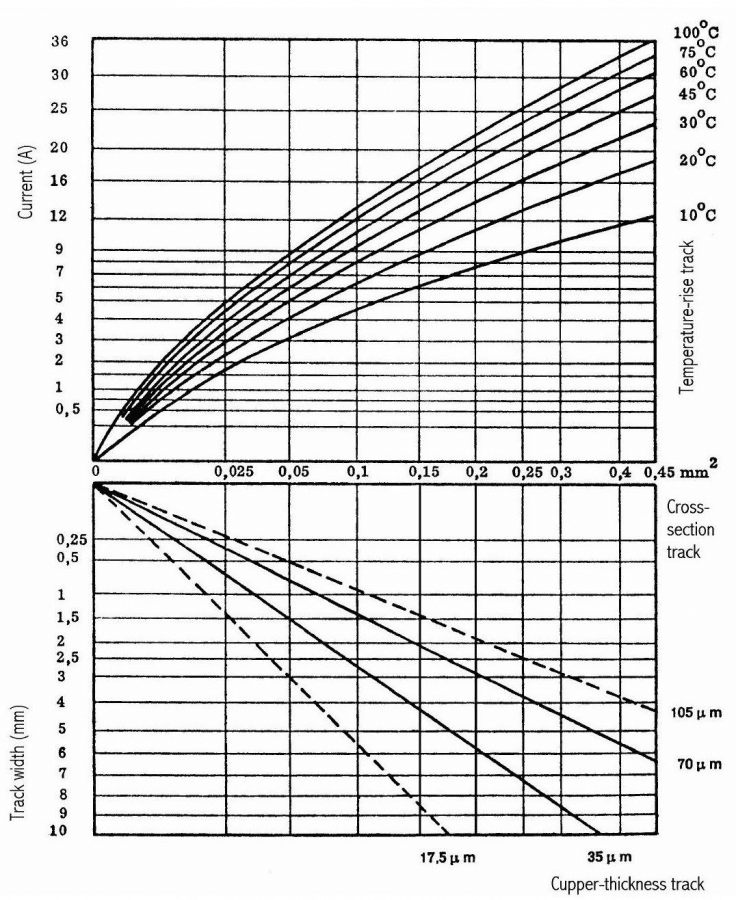
\includegraphics[width=0.45\textwidth]{track-width.png} &
			
			\begin{enumerate}
				\item Zvolím proud a oteplení,
				\item najdu požadovaný průřez,
				\item ze spodního grafu najdu pro konkrétní tloušťku vrstvy požadovanou šířku spoje dle průřezu.
			\end{enumerate}
		\end{tabular}
	\end{center}
	
\end{frame}

%------------------------------------------------------------------------------
\begin{frame}
	\frametitle{Omezení návrhu - izolační vzdálenost}
	
	\begin{center}
		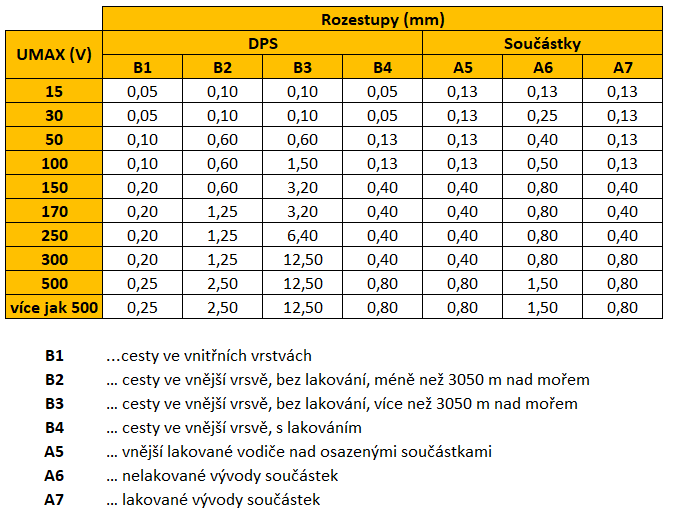
\includegraphics[width=0.8\textwidth]{spacing.png}
	\end{center}
	
\end{frame}
%------------------------------------------------------------------------------
\begin{frame}
	\frametitle{Zdroje dat}

	\begin{enumerate}
		\item http://www.isola-group.com/wp-content/uploads/
		\item https://www.youtube.com/watch?v=z4f-D1EKKD4
		\item https://www.youtube.com/watch?v=T7S40GYESbY
		\item https://www.youtube.com/watch?v=hpR4e1n0HKo\&t=204s
	\end{enumerate}
\end{frame}
%------------------------------------------------------------------------------

\end{document}